%!TEX root = ../main.tex

\subsection{Ablation Studies of \texttt{GoodCore}$^+$}
\noindent{\bf Hyperparamaters for grouping.}

\begin{figure}
	\centering
	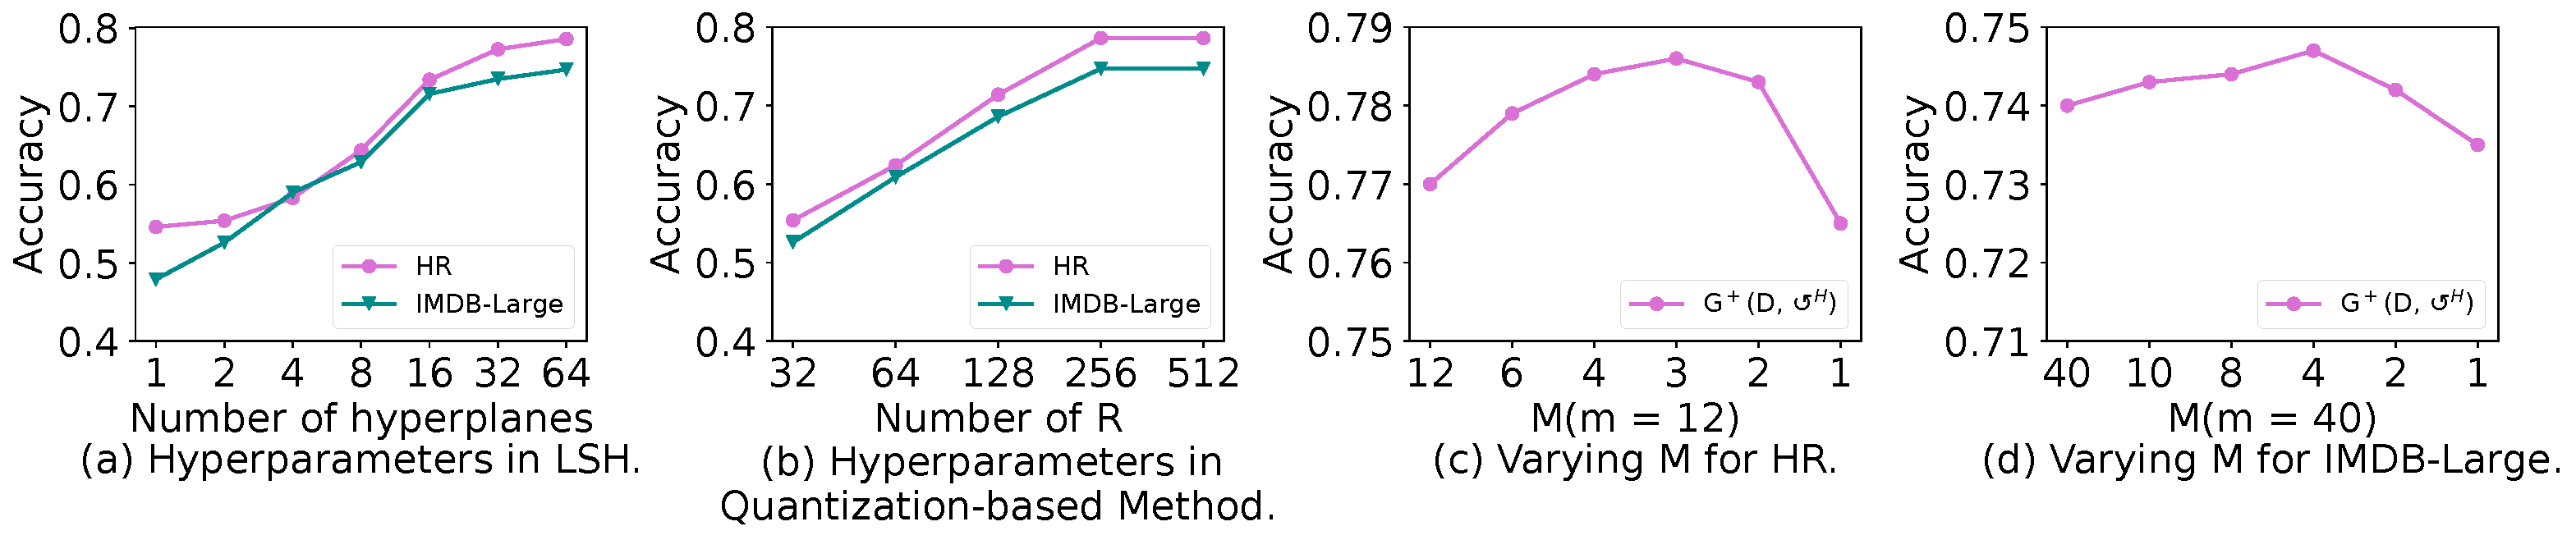
\includegraphics[width=1\textwidth]{figs/M}
	\vspace{-1em}
	\caption{Varying Hyperparameters in LSH and Quantization-based Method.}
	\label{fig:pq-exp}
	\vspace{-1em}
\end{figure}

We use LSH to efficiently group the entire dataset, and test the impact of  different numbers of hyperplanes, which is a significant parameter in LSH.
 As shown in Figure~\ref{fig:pq-exp} (a), with the number increasing, more groups are generated, and the tuples within each cluster are closer, so the  accuracy increases at the beginning. Afterwards, the accuracy remains stable because tuples in each cluster are similar enough for  approximating the gradient. Therefore, empirically, using  64 hyperplanes is the most appropriate because more groups will reduce the efficiency.

\noindent{\bf Hyperparamaters in Quantization-based Method.} In Section~\ref{subsec:pq}, we use quantization-based method to estimate the upper bound $\hat{s}_{ju}$ of $\overline{s}_{ju}$. Recap that \texttt{GoodCore}$^+$ needs the user-specified cluster centers size $R$, which is important for computing the maximum feature distances.
%
 To choose a proper $R$, we adopt a simple yet effective solution that selects different $R$ and obtain different coresets. Then we train over these coresets and evaluate via a validation set to get different results. Specifically, we select $R$ from 32 to 512 for each dataset. Figure~\ref{fig:pq-exp} (b) shows the performance on dataset \hr and \imdbl when varying the cluster centers size $R$.  We can see that as $R$ increases, the accuracy of the dataset also gradually increases, because when $R$ increases, the upper bound $\hat{s}_{ju}$ is closer to $\overline{s}_{ju}$, which can help us to select a good coreset.


We also test the performance of different feature splitting ways (corresponding to different $M$). In Figure~\ref{fig:pq-exp}(c)-(d), initially,  $M=12$ indicates that in each subspace, the length of all sub-vectors is 1. With $M$ decreasing, the accuracy increases first because each sub-vector becomes longer, which contains more information when adding up these $\hat{s}^z_{ju}$, leading to a more precise bound. But if each sub-vector is too long, which means that each vector is quantized to a very short code, the accuracy decreases because in this situation, the quantization-based method is not informative enough to give accurate  distance estimation. Empirically, when $M$ is around 3, it is always a good choice.
